\documentclass[a4paper,12pt]{report}
\usepackage[portuguese]{babel}
\usepackage[latin1]{inputenc} 
\usepackage{amssymb}
\usepackage{listings}
\usepackage{graphicx}
\usepackage{anysize}
\usepackage{booktabs}
\usepackage{hyperref}

\begin{document}

\title{Compiladores\\Trabalho 4 - S\'intese}
\author{Jackson Willian Brito; Talles Tatagiba Martins de Souza}
\date{Mar\c{c}o, 2014}
\maketitle

\pagebreak

\tableofcontents

\pagebreak

\renewcommand{\thesection}{\arabic{section}} 

\begin{abstract}
Neste relat\'orio detalha-se todo o processo de cria\c{c}\~ao de um interpretador da linguagem G-Portugol incluindo as etapas de an\'alise e suas 3 fases e a etapa de s\'intese para a disciplina Compiladores bem como apresenta as considera\c{c}\~oes feitas pelos autores do trabalho a fim de garantir integridade na linguagem.
\end{abstract}

\section{Introdu\c{c}\~ao}

Da literatura, temos a defini\c{c}\~ao de um compilador como sendo um programa que recebe um programa escrito em uma linguagem
fonte e o transforma em um programa em uma linguagem destino. Os programas fonte e alvo devem ter o mesmo significado. Uma caracter\'istica
imprescind\'ivel de um compilador \'e a capacidade de detectar e reportar erros.

O processo de compila\c{c}\~ao pode ser subdividido nas etapas de an\'alise e s\'intese. A etapa de an\'alise pode ser subdividida em 
3 fases, s\~ao elas: l\'exica, sint\'atica e sem\^antica. Neste trabalho abordamos a etapa de s\'intese sobre as tr\^es fases de anz'alise desenvolvidas anteriormente. Aqui \'e apresentado um apanhado completo da constru\c{c}\~ao de um compilador.

Ao fim deste pretende-se ter um interpretador da varia\c{c}\~ao da linguagem G-Portugol
aqui apresentada. 

\section{A linguagem - G-Portugol}

Para a elabora\c{c}\~ao do trabalho de compiladores foi escolhida como linguagem dos programas fontes do nosso compilador a
linguagem G-Portugol que \'e uma linguagem voltada ao ensino inicial de programa\c{c}\~ao e por isso n\~ao possui bem definida e
formatada todas as suas estruturas. Assim, para completar o processo de compila\c{c}\~ao foram inseridas caracter\'isticas
pr\'oprias de outras linguagens de programa\c{c}\~ao conceituadas tendo e assim constru\'ir um interpretador capaz de reconhecer programas escritos nesta varia\c{c}\~ao da linguagem
G-Portugol, executá-lo ou reportar erros, quando houver.

\section{An\'alise l\'exica}

A an\'alise l\'exica consiste na identifica\c{c}\~ao de $tokens$ da linguagem fonte dentro do arquivo de entrada. 
Nesta fase a gram\'atica da linguagem \'e verificada. Um analisador l\'exico \'e capaz de reconhecer uma gram\'atica 
atrav\'es de um aut\^omato finito.

Faz-se necess\'ario frizar que n\~ao houve o desenvolvimento de um analisador l\'exico, apenas a forma\c{c}\~ao das regras 
atrav\'es das quais a ferramenta computacional $flex$ construiu o analisador.

\subsection{Flex}

$Flex$ \'e uma ferramenta computacional que, a partir da especifica\c{c}\~ao de regras gramaticais por meio de express\~oes
regulares, gera um programa em $c$ capaz de reconhecer palavras que obedecem as regras estabelecidas ($tokens$).

\subsection{Palavras reservadas}

As palavras reservadas da nossa linguagem s\~ao basicamente as palavras reservadas que aparecem no manual de G-Portugol 
acrescidas das palavras necess\'arias para construir as estruturas n\~ao contempladas pelo manual.

Abaixo seguem listadas todas as palavras reservadas da linguagem em ordem alfab\'etica.
\begin{itemize}
\item algoritmo
\item at\'e
\item caractere
\item caracteres
\item caso
\item de
\item e
\item enquanto
\item ent\~ao
\item fa\c{c}a
\item falso
\item fim
\item fim-enquanto
\item fim-fa\c{c}a
\item fim-para
\item fim-se
\item fim-seleciona
\item fim-vari\'aveis
\item fun\c{c}\~ao
\item in\'icio
\item inteiro
\item inteiros
\item literais
\item literal
\item l\'ogico
\item l\'ogicos
\item matriz
\item n\~ao
\item ou
\item para
\item parar
\item passo
\item reais
\item real
\item retorne
\item se
\item seleciona
\item sen\~ao
\item vari\'aveis
\item verdadeiro
\end{itemize}


\subsection{N\'umeros}

Para o reconhecimento de n\'umeros com sinais por exemplo, pode-se optar por reconhec\^e-los com sinais na fase de an\'alise
l\'exica e inferir a opera\c{c}\~ao na an\'alise sem\^antica; ou reconhecer n\'umeros e operadores separadamente e posteriormente, 
na fase de an\'alise sem\^antica, identificar a sequ\^encia $operador-numero$ como sendo, em realidade um n\'umero com sinal.

Optou-se, nesta implementa\c{c}\~ao reconhecer apenas os numerais antecedidos pelo s\'imbolo de 
negativo como n\'umeros na fase de analise l\'exica, sendo assim imposs\'ivel representar um n\'umero como $+1$ por exemlo, apesar de a nota\c{c}\~ao $-1$ ser admiss\'ivel.

\subsubsection{Real}
Outra escolha importante \'e a forma como ser\~ao representados os n\'umeros reais. No manual de portugol ele reconhece apenas
d\'igitos seguidos de ponto seguido por d\'igitos.
Nossa varia\c{c}\~ao da linguagem torna opcional o acr\'escimo da letra $e$ ou $E$ seguida, opcionalmente, por um sinal seguido obrigatoriamente por d\'igitos, sendo
poss\'ivel assim representar pot\^encias de $10$.

S\~ao portanto exemplos de n\'umeros reais reconhecidos por nosso analisador:
\begin{itemize}
 \item 10.0
 \item -10.0
 \item 10.10E10
 \item -10.10
 \item -10.10e1
 \item 10.11e-2
\end{itemize}


\subsection{Coment\'arios}

\subsubsection{Linha}

A defini\c{c}\~ao de coment\'arios de linha s\~ao quaisquer sequ\^encias de caracteres 
escritos depois de ``//'' que n\~ao seja o avan\c{c}o de linha ($\backslash$n).

\subsubsection{Bloco}

A defini\c{c}\~ao de coment\'rios por blocos se inicia por (/*) e termina necessariamente por (*/), 
sendo que quaisquer sequ\^encias de caracteres entre os s\'imbolos aqui definidos s\~ao 
ignorados pelo compilador.

Foi utilizado, ao final, o c\'odigo cedido pela professora para avali\c{c}\~ao de coment\'arios de bloco e contagem de linhas a fim de retornar o valor exato da linha em caso de existir algum erro. 

\section{An\'alise sint\'atica}

A an\'alise sint\'atica consiste na cria\c{c}\~ao das regras de forma\c{c}\~ao da gram\'atica da linguagem fonte e 
posterior compara\c{c}\~ao do arquivo fonte entregue para estabelecer se o mesmo est\'a corretamente escrito
na liguagem fonte. Caso o arquivo fonte n\~ao esteja corretamente escrito na linguagem fonte deve-se
reportar um erro indicando a linha na qual est\'a a diverg\^encia entre o escrito e o que se esperava para
que estivesse corretamente redigido na linguagem esperada.

\'e de suma import\^ancia frizar que n\~ao houve o desenvolvimento de um analisador sint\'atico, mas sim a 
utiliza\c{c}\~ao da ferramenta computacional $bison$ que gera o analisador sint\'atico partindo das regras
da gram\'atica esperada, estas sim definidas por n\'os e descritas neste relat\'orio.


\subsection{Bison}

$Bison$ \'e uma ferramenta computacional que, a partir das regras sint\'aticas da gram\'atica a qual se busca
aceitar, constroi um analisador sint\'atico que percorre o arquivo de entrada tentando encaixar o que est\'a
no arquivo com suas regras, caso n\~ao consiga realizar este casamento, invoca uma fun\c{c}\~ao de erro.

\subsection{Programa vazio}

Para a nossa linguagem o menor programa pass\'ivel de reconhecimento \'e o descrito abaixo

\begin{verbatim}
algoritmo nome_do_algoritmo;

inicio

fim
\end{verbatim}

\subsection{Comandos de sele\c{c}\~ao}

\subsubsection{Se-ent\~ao e Se-ent\~ao-sen\~ao}

A estrutura do comando de sele\c{c}\~ao Se-ent\~ao-sen\~ao \'e apresentada abaixo.
A presen\c{c}a do sen\~ao \'e opcional e \'e poss\'ivel aninha-los.

\begin{verbatim}
se (CONDICAO) entao 
	BLOCO
fim-se
\end{verbatim}
ou
\begin{verbatim}
se (CONDICAO) entao 
	BLOCO
senao
	BLOCO
fim-se
\end{verbatim}

\subsubsection{Seleciona-caso}

No exemplo abaixo FATOR\_CASE s\~ao os primitivos que o switch aceita como comparadores e s\~ao eles:
inteiro, real e caracter.
O caso padr\~ao, que \'e executado se nenhum caso anterior for atendido, \'e opcional.

\begin{verbatim}
seleciona (IDENTIFICADOR)
	caso (FATOR_CASE): BLOCO parar;
    caso (FATOR_CASE): BLOCO
    caso (FATOR_CASE): BLOCO parar;
    	...
    padrao: BLOCO parar;
fim-seleciona
\end{verbatim}

\subsection{Comandos de repeti\c{c}\~ao}

\subsubsection{Enquanto}

An\'alogo ao $While$ em C/Java;

\begin{verbatim}
enquanto (CONDICAO)
	BLOCO
fim-enquanto
\end{verbatim}

\subsubsection{Fa\c{c}a-enquanto}

An\'alogo ao $Do-while$ em C/Java;

\begin{verbatim}
faca
	BLOCO
fim-faça enquanto (CONDICAO);
\end{verbatim}

\subsubsection{Para}

An\'alago ao $For$ em C/Java;

\begin{verbatim}
para (VARIAVEL de VALOR_INICIAL ate CONDICAO passo PASSO) faca
	BLOCO
fim-para
\end{verbatim}

\subsection{Declara\c{c}\~ao de vari\'aveis}

As declara\c{c}\~oes de vari\'aveis devem ser feitas em local devido. Ap\'os o nome e antes do in\'icio tanto do programa principal quanto de fun\c{c}\~oes.

Deve seguir a seguinte sintaxe:

\begin{verbatim}
variaveis
	IDENTIFICADOR : TIPO;
	IDENTIFICADOR : matriz[INTEIRO] de TIPO_PLURAL;  //para vetores
    IDENTIFICADOR : matriz[INTEIRO][INTEIRO] de TIPO_PLURAL;  //para matrizes
fim-variaveis
\end{verbatim}

A linguagem reconhece apenas a declara\c{c}\~ao de vetores (matrizes unidimensionais) e matrizes (bidimensionais).

\subsection{Inicializa\c{c}\~ao de vari\'aveis}

O interpretador exigem que todas as vari\'aveis, antes de terem seu valor utilizado tenham 
sofrido atribui\c{c}\~ao para evitar lixo de mem\'oria.

\subsection{Declara\c{c}\~ao de fun\c{c}\~oes}

Especificou-se que todas as fun\c{c}\~oes devem ser declaradas antes do início do BLOCO\_PRINCIPAL.
A seguir a estrutura para declara\c{c}\~ao de fun\c{c}\~ao.

\begin{verbatim}
//funcao com retorno
funcao NOME( ARGUMENTO : TIPO_DO_ARGUMENTO ) : TIPO_DA_FUNCAO
	DECLARACAO_DE_VARIAVEIS
inicio
	BLOCO
fim
\end{verbatim}
ou
\begin{verbatim}
//funcao sem retorno
funcao NOME( ARGUMENTO : TIPO_DO_ARGUMENTO )
	DECLARACAO_DE_VARIAVEIS
inicio
	BLOCO
fim
\end{verbatim}


\subsection{Atribui\c{c}\~ao \`a variaveis}

Valores as vari\'aveis podem ser atribu\'idos da seguinte forma:

\begin{verbatim}
	IDENTIFICADOR := EXPRESSAO;
\end{verbatim}

\subsection{Comandos}

O corpo do programa \'e constituido por uma sequencia de comandos que podem ser atribui\c{c}\~oes ou comandos de sele\c{c}\~ao ou repeti\c{c}\~ao.

\section{An\'alise sem\^antica}

A an\'alise sem\^antica consiste na varredura do programa de entrada representa de fato
um programa v\'alido na linguagem fonte atentando-se as regras de escrita da linguagem e 
as restri\c{c}\~oes de tipos e operadores. Nesta etapa s\~ao constru\'idas as estruturas de
controles de varia\'aveis e fun\c{c}\~oes nas quais constar\~ao dados sem\^anticos tais como
escopo, tipo, aridade, entre outros que ser\~ao analisados. Caso o arquivo fonte n\~ao esteja 
escrito de maneira semanticamente correta na linguagem fonte deve-se
reportar um erro indicando a linha na qual est\'a a diverg\^encia entre o escrito e o que 
se esperava para que estivesse, o programa, corretamente redigido na linguagem esperada.

\'E de suma import\^ancia frizar que ao contr\'ario da etapa de an\'alise l\'exica e 
sint\'atica, nas quais fizemos uso de ferramentas computacionais para realiza\c{c}\~ao das 
mesmas, nesta etapa, apesar do uso das ferramentas como suporte, toda a l\'ogica de an\'alise
foi desenvolvida por n\'os.

\subsection{Express\~oes}

Conforme especifica\c{c}\~ao express\~oes n\~ao incluem, exceto em atribui\c{c}\~oes, literais 
ou caracteres. Mas incluem vari\'aveis, acessos a posi\c{c}\~oes de matrizes, chamadas de 
fun\c{c}\~oes e n\'umeros inteiros e reais, todos precedidos ou n\~ao de sinais indicativo de 
n\'umero negativo. Ainda reconhece express\~oes l\'ogicas com operadoes de compara\c{c}\~ao e 
operadores l\'ogicos.

No que tange a compara\c{c}\~oes l\'ogicas vale ressaltar que para efeito de an\'alises
destas nosso analisador sem\^antico entende que um n\'umero pode ser considerado um 
l\'ogico adotando a convers\~ao: 0 - $falso$ | n\~ao 0 - $verdadeiro$.

\'E v\'alido ressaltar que todos os operadores definidos ($+$,$-$,$*$,$/$,$<$,$>$,$e$, $ou$ e 
outros) s\'o podem ser executados sobre operandos de mesmo tipo e para os tipos que n\~ao sejam
caracter ou literal, ou matrizes de qualquer tipo sem sele\c{c}\~ao de posi\c{c}\~ao.

\subsection{Estruturas de sele\c{c}\~ao e repeti\c{c}\~ao}

Estruturas de sele\c{c}\~ao aceitam express\c{c}\~oes que retornem valores l\'ogicos, seja 
apenas uma vari\'avel, as palavras reservadas $verdadeiro$ e $falso$ ou express\~oes complexas
cujo resultado seja um l\'ogico.

Comandos de la\c{c}o avaliam express\~oes l\'ogicas similarmente \`a estrutura de sele\c{c}\~ao
na parte condicional.

\'E de bom tom frizarmos que para o comando $selecione$ os tipos inseridos dentro de um $caso$ 
devem ser o mesmo da vari\'vel usada para compara\c{c}\~ao, caso contr\'ario, pela pr\'opria 
restri\c{c}\~ao feita em express\~oes, a compara\c{c}\~ao n\~ao poder\'a ser feita, sendo assim 
um erro sem\^antico que ser\'a acusado pelo nosso compilador. Ainda nessa caminho, as 
itera\c{c}\~oes autom\'aticas do la\c{c}o $fa$\c{c}$a$ devem ser definidas sobre os mesmo
tipos, tamb\'em respeitando as restri\c{c}\~oes impostas ao operador de 
adi\c{c}\~ao/subtra\c{c}\~ao.

\subsection{Tipos de vari\'aveis}

A linguagem aceita pelo interpretador possui 5 tipos, s\~ao eles:

\begin{itemize}
	\item inteiro
    \item real
    \item caracter
    \item literal
    \item l\'ogico
\end{itemize}

As precis\~oes utilizadas foram $int$ para inteiro, $double$ para real e $char$ para caracter,
literais são alocados como vetores de $char$ de tamanho 50, sendo ent\~ao este o limite para 
todo e qualquer literal utilizado na linguagem. Os valores l\'ogicos s\~ao tamb\'em 
representados como $int$;

\subsection{Declara\c{c}\~ao de vari\'aveis}

As declara\c{c}\~oes de vari\'aveis devem ser feitas em local apropriado no princ\'ipio do 
programa ou no in\'icio de uma fun\c{c}\~ao. O formato padr\~ao para declara\c{c}\~ao \'e $identificador$ seguido por $dois pontos$ seguido do tipo.

\begin{verbatim}
//Exemplor de declaracao de variaveis
a : inteiro;
b : real;
c : caracter;
d : literal;
e : logico;
\end{verbatim}

Nesta etapa, quando identificada uma declara\c{c}\~ao de vari\'avel criamos um registro dessa vari\'avel identificado pelo seu nome e seu escopo e tamb\'em alocamos o espa\c{c}o necess\'ario para guardar o valor da mesma. No caso de matrizes s\~ao guardadas tamb\'em sua dimens\~ao e a quantidade de itens em cada uma. Essa estrutura \'e ent\~ao guardada em uma hash.

\subsection{Atribui\c{c}\~ao \`a vari\'aveis}

No momento da atribui\c{c}\~ao de uma express\~ao a uma vari\'avel faz-se a checagem dos tipo 
da vari\'avel e da express\~ao para saber se s\~ao compat\'iveis o que s\'o pode ocorrer se a 
vari\'avel em quest\~ao tiver sido previamente declarada no bloco em que est\'a sendo 
utilizada, que \'e o alvo da primeira verifica\c{c}\~ao feita.

\subsection{Inicializa\c{c}\~ao de vari\'aveis}

No momenta da atribui\c{c}\~ao, caso n\~ao tenha ocorrido erro, a vari\'avel \'e identificada como possuindo um valor v\'alido, permitindo assim que a mesma tenha seu valor utilizado em outras express\~oes.

Caso uma vari\'avel seja declarada e n\~ao tenha seu valor inicializado corretamente em nenhum lugar do programa \'e emitido um Aviso para o programador.

\subsection{Declara\c{c}\~ao de fun\c{c}\~ao}

Ao encontrar uma fun\c{c}\~ao gera-se uma estrutura de controle identificada pelo nome e contendo informa\c{c}\~oes importantes de controle tais como os par\^ametros, suas vari\'aveis e a sequencia de comandos que a identifica.

\'E ainda verificado se h\'a o comando $retorne$ em fun\c{c}\~oes especificadas como possuindo retorno.

\subsection{Aridades de fun\c{c}\~ao}

Ao verificar a declara\c{c}\~ao de uma fun\c{c}\~ao \'e feito ainda a contagem dos par\^ametros 
que a mesma recebe definindo assim sua aridade que \'e conferida a cada invoca\c{c}\~ao da mesma
acusando erro em caso de falta ou excesso de par\^ametros.

\subsection{Matrizes}

Matrizes s\~ao tratadas como um tipo especial de vari\'avel, tendo na sua 
estrutura uma flag indicando que se trata de uma matriz e as informa\c{c}\~oes referente a 
dimens\~ao e n\'umero de linhas e colunas.

\subsubsection{Declara\c{c}\~ao e tipos}
Matrizes podem ser de 4 tipos:
\begin{itemize}
	\item de inteiros
    \item de reais
    \item de caracteres
    \item de literais
\end{itemize}

Podemos declar\'a-las conforme a seguinte sintaxe:

\begin{verbatim}
//Declaracao de matrizes/vetores
m[2][2] : de inteiros;
n[2] : de reais;
o[3][5] : de caracteres;
p[7] : de literais;
\end{verbatim}

\subsubsection{Inicializa\c{c}\~ao}

Para matrizes h\'a duas formas de realizar a atribui\c{c}\~ao de valores para suas 
posi\c{c}\~oes, descritas descritas a seguir. Apenas a atribui\c{c}\~ao completa realiza
a inicializa\c{c}\~ao correta da matriz, validando assim seus valores frente as demais ocorr\^encias no programa.

\subsubsection{Atribui\c{c}\~ao completa}

A atribui\c{c}\~ao completa de um vetor (matriz de dimens\~ao 1) deve ser realizada da seguinte 
forma:

\begin{verbatim}
	//Exemplo para um vetor de 5 literais
	mat = ["Ahh","Ehh","Ihhhh","oh","Uhhh"];
\end{verbatim}

J\'a para uma matriz de dimens\~ao 2 deve-se proceder da seguinte maneira:

\begin{verbatim}
	//Exemplo para uma matriz[5][2] de inteiros
	mat = {[1,2,3,4,5],[6,7,8,9,10]};
\end{verbatim}

\subsubsection{Atribui\c{c}\~ao a posi\c{c}\~ao espec\'ifica}

Pode-se atribuir uma express\~ao, cujo resultado seja do mesmo tipo da matriz, a uma posi\c{c}\~ao espec\'ifica da matriz da forma mostrada a seguir:

\begin{verbatim}
	//Exemplo para uma matriz de inteiros
	mat[0][0] := 10+7;
\end{verbatim}

Ressaltando que neste momento \'e feita verifica\c{c}\~ao do tamanho de cada dimens\~ao da
matriz, evitando assim atribui\c{c}\~oes a espa\c{c}os de mem\'oria err\^oneos.

\subsubsection{Uso em express\~oes}

Pode-se acessar uma posi\c{c}\~ao espec\'ifica da matriz
utilizando-a como parte de uma express\~ao conforme exemplo a seguir:

\begin{verbatim}
	//Exemplo para uma matriz de inteiros
    //variavel a  inteira
	a := 10 + mat[0][0];
\end{verbatim}


\section{S\'intese}

A etapa de s\'intese consiste em enla\c{c}ar os resultados obtidos nas diversas fases da etapa
de an\'alise e agregar a l\'ogica necess\'aria para seu devido funcionamento.

Primeiramente, no momento da compila\c{c}\~ao \'e gerada a \'arvore de execu\c{c}\~ao de cada comando e esta \'e colacada em uma fila (FIFO). Caso não seja encontrado erros em nenhuma das etapas de an\'alise a fila de \'arvores resutante ser\'a a fila a ser executada pelo interpretador.

A maneira de montar cada \'arvore varia de acordo com os comandos utilizados, entretanto, em ess\^encia devem ter em sua ra\'iz a opera\c{c}\~ao representada e em suas folhas os fatores componentes da mesma.

\subsection{N\'o da \'arvore de execu\c{c}\~ao}

Para representar a menor divis\~ao poss\'ivel de cada comando usamos, como pode ser verificado na figura \ref{fig:No}, uma estrutura que identifica seu tipo, seu valor e, para poder ser organizada em \'arvore e em pilha atendendo as necessidades previamente levantadas possui 5 ponteiros sendo 4 usados como filhos e 1 como pr\'oximo.

\begin{figure}
\centering
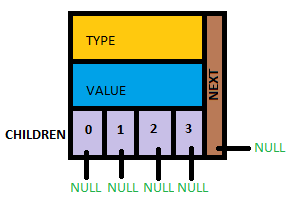
\includegraphics[width=0.3\textwidth]{imgs/Estrutura_b_sica.png}
\caption{\label{fig:No}Estrutura b\'asica da \'arvore de execu\c{c}\~ao.}
\end{figure}

\subsection{Tipos primitivos}

G-Portugol aceita declara\c{c}\~ao de vari\'aveis de 5 tipos, a saber: $inteiro$, $real$, $caracter$, $literal$ e $l$\'o$gico$. Cata tipo possui seu valor atribuido ao campo $value$ e seu tipo \'e contido no campo $type$. Conforme ilustrado na figura \ref{fig:fatores}.

\begin{figure}
\centering
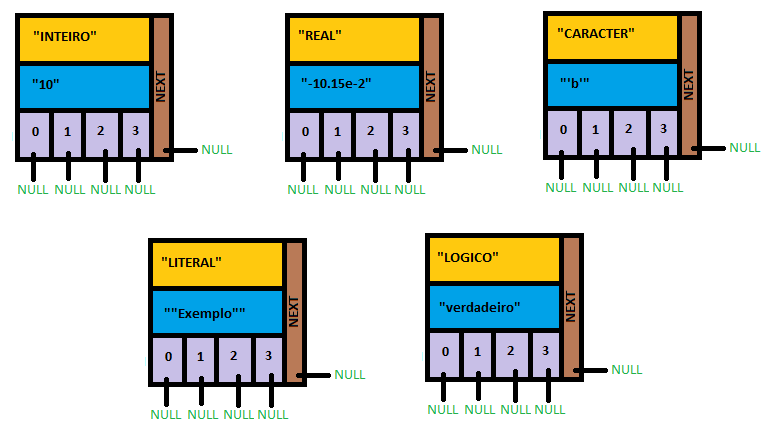
\includegraphics[width=0.8\textwidth]{imgs/Tipos_primitivos.png}
\caption{\label{fig:fatores}Estrutura de execu\c{c}\~ao montada para os tipos primitivos da linguagem.}
\end{figure}

\subsection{Vari\'aveis}

Vari\'aveis possuem $type$ = "VARIAVEL" e em $value$ possue o nome utilizado para identific\'a-la na hash de vari\'aveis. Ver figura \ref{fig:variaveis}.

\begin{figure}
\centering
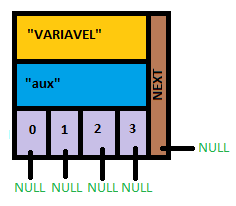
\includegraphics[width=0.3\textwidth]{imgs/Variavel.png}
\caption{\label{fig:variaveis}Estrutura de execu\c{c}\~ao montada paravari\'aveis.}
\end{figure}

\subsection{Fun\c{c}\~oes}
As fun\c{c}\~oes s\~ao inicializadas no in\'cio do programa e seus respectivos n\'os de \'arvore t\^em o formato definido na figura \ref{fig:funcoes}.

\begin{figure}
\centering
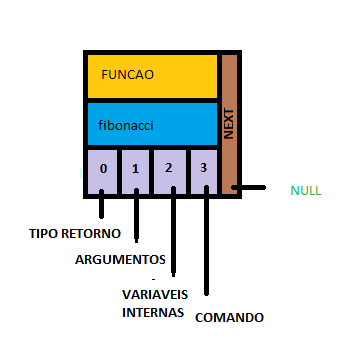
\includegraphics[width=0.3\textwidth]{imgs/funcao.png}
\caption{\label{fig:funcoes}Estrutura de execu\c{c}\~ao montada para fun\c{c}\~oes.}
\end{figure}

Dentro da estrutura de fun\c{c}\~oes do programa que \'e armazenada na respectiva tabela \i{hash} de fun\c{c}\~oes, ir\'a possuir um ponteiro para a \'arvore que ser\'a espertamente utilizado durante o programa para cada vez que precisarmos acessar a fun\c{c}\~ao.
O primeiro n\'o da \'arvore aponta para outro n\'o que cont\'em o tipo de retorno da fun\c{c}\~ao. O segundo filho aponta para o n\'o que cont\'em uma lista de n\'os atrav\'es do \i{next} de todos os argumentos da fun\c~ao. O terceiro filho cont\'em as vari\'aveis internas utilizadas dentro da fun\c{c}\~ao no mesmo esquema anterior e o quarto filho cont\'em o COMANDO que pode conter qualquer outra coisa de acordo com a sintaxe da linguagem.


\subsubsection{Chamadas de Fun\c{c}\~ao}

Durante a execu\c{c}\~ao do programa, ocorrem as chamadas de fun\c{c}\~ao. Nestas chamadas, um novo n\'o de \'arvore \'e criado na \'arvore do programa para posterior execu\c{c}\~ao. Este n\'o possui o formato apresentado na figura \ref{fig:chamadafuncao}.

\begin{figure}
\centering
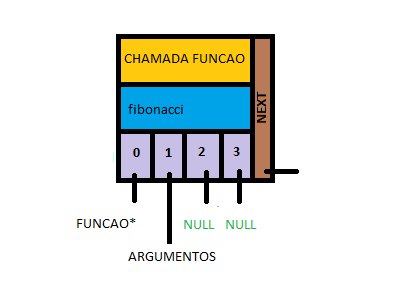
\includegraphics[width=0.3\textwidth]{imgs/chamada_funcao.png}
\caption{\label{fig:chamadafuncao}Estrutura de execu\c{c}\~ao montada para chamada de fun\c{c}\~oes.}
\end{figure}

O primeiro n\'o da chamada de fun\c{c}\~ao aponta para o n\'o da fun\c{c}\~ao criado, por\'em um recurso especial foi utilizado para correta exibi\c{c}\~ao no caso de recurs\~ao, para isto, o filho do COMANDO na fun\c{c}\~ao \'e apontado para NULL.
O segundo n\'o da chamada de fun\c{c}\~ao aponta para os argumentos chamados de uma maneira a facilitar a posterior execu\c{c}\~ao. Neste novo n\'o criado, os dois primeiros filhos da lista de n\'os contendo os argumentos, ser\~ao respectivamente a express\~ao que est\'a sendo passada na fun\c{c}\~ao e o argumento da fun\c{c}\~ao correspondente.


\subsection{Posi\c{c}\~ao em Matrizes},

Similar a vari\'aveis, mas contendo "MATRIZ" no $type$ e contendo nos filhos 0 e 1 inteiros que indicam respectivamente a coluna e a linha acessadas. Sua estrutura pode ser verificada na figura \ref{fig:matriz}.

\begin{figure}
\centering
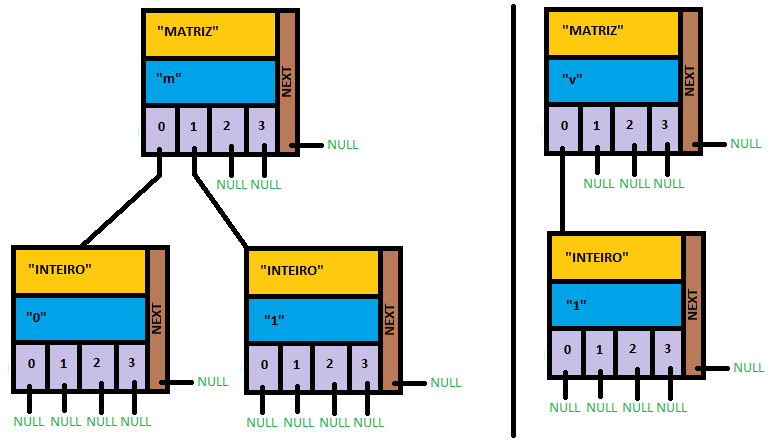
\includegraphics[width=0.8\textwidth]{imgs/Matriz.png}
\caption{\label{fig:matriz}Estrutura montada a partir do acesso a uma posi\c{c}\~ao da matriz.}
\end{figure}

\subsection{Operadores}

Existem 5 grupos de operadores segundo sua ordem de precedencia, são eles:

\begin{description}
\item[Operadores de nivel 3] $e$, $ou$ - menor precedencia;
\item[Operadores de nivel 2] $<$, $<=$, $>$, $>=$, =, $<>$; 
\item[Operadores de nivel 1] +,-;
\item[Operadores de nivel 0] *,/,\%;
\item[Operadores de menor nivel] \^ - maior precedencia;
\end{description}

As estruturas montadas para os repesentantes de cada grupo estão detalhadas na figura \ref{fig:operadores}.

\begin{figure}
\centering
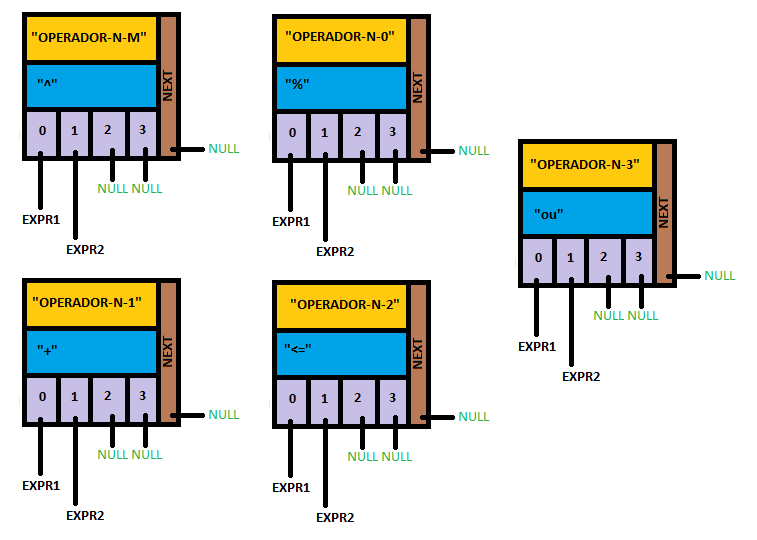
\includegraphics[width=0.8\textwidth]{imgs/Operadores.png}
\caption{\label{fig:operadores}Estrutura montada a partir dos operadores.}
\end{figure}

\subsection{Express\~oes}

Express\~oes podem ser formadas por fatores de tipos primitivos, vari\'aveis, posi\c{c}\~oes de matrizes, fun\c{c}\~oes ou outras express\~oes entre par\^entesis.

\subsubsection{Parentesis}

Um express\~ao destacada por par\^entesis tem sua precedencia elevada em rela\c{c}\~ao a express\~ao da qual faz parte, devendo assim ser executada primeiro (o que significa ser al\c{c}ada ao topo da \'arvore). Para representar a esistencia de par\^entesis delimitando a express\~ao a estrutura apresentada na figura \ref{fig:parentesis} foi montada.

\begin{figure}
\centering
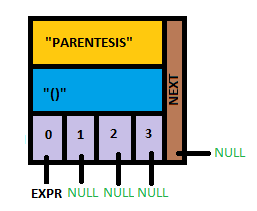
\includegraphics[width=0.3\textwidth]{imgs/Parentesis.png}
\caption{\label{fig:parentesis}Estrutura montada a partir dos parentesis.}
\end{figure}

\subsection{Atribui\c{c}\~oes}

Atribui\c{c}\~oes possuem representados a vari\'avel ou posi\c{c}c\~ao de matriz a qual o valor resultado da express\~ao deve ser atribuido e a dita express\~ao. Representada conforme figura \ref{fig:atribuicoes}.

\begin{figure}
\centering
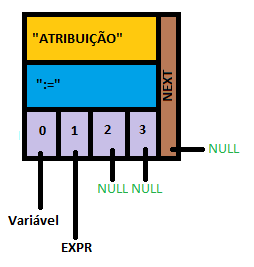
\includegraphics[width=0.3\textwidth]{imgs/Atribui__p.png}
\caption{\label{fig:atribuicoes}Estrutura montada a partir de uma atribui\c{c}\~ao.}
\end{figure}

\subsection{Enquanto e Fa\c{c}a-enquanto}

Ambas cont\'em a condi\c{c}\~ao de parada e o bloco de comando a ser executado. Lembrando que por bloco de comando se entende uma lista de n\'os de comandos. Ver figura \ref{fig:enquanto}.

\begin{figure}
\centering
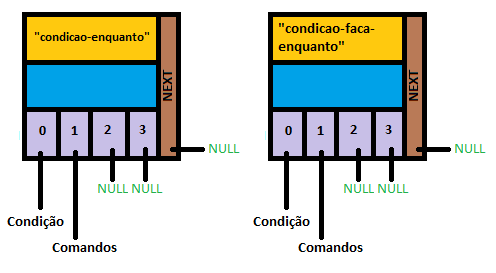
\includegraphics[width=0.5\textwidth]{imgs/enquanto_e_faca-enquanto.png}
\caption{\label{fig:enquanto}Estruturas montadas a partir dos comandos enquanto e fa\c{c}a-enquanto.}
\end{figure}

\subsection{Seleciona}

O comando seleciona, conforme apresentado na figura \ref{fig:seleciona}, possui como primeiro filho a vari\'avel que deseja comparar e no segundo uma lista contendo todos os casos e terminados pelo caso padr\~ao quando este existir.

Cada estrutura caso possui como primeiro filho o valor a ser comparado e como segundo o comando a ser executado e no terceiro pode ou n\~ao haver o comando parar, indicando se deve ser interrompido ou seguir para o caso seguinte.

\begin{figure}
\centering
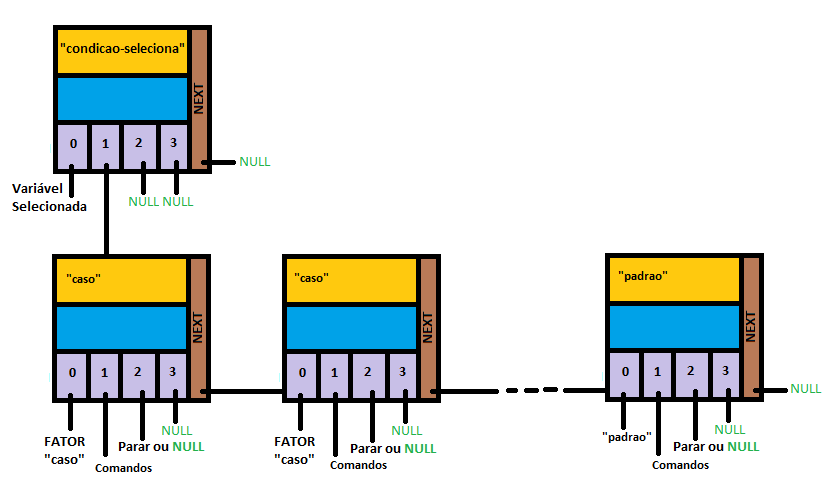
\includegraphics[width=0.8\textwidth]{imgs/Seleciona.png}
\caption{\label{fig:seleciona}Estrutura montada a partir do comando seleciona.}
\end{figure}

\subsection{Para}

Para o comando $para$ a estrutura montada possue em seu primeiro filho a atribui\c{c}\~ao necess\'aria para dar in\'icio ao comando, seguido pelo filho que realiza a copara\c{c}\~ao deste com o fator at\'e, no terceiro filho h\'a a atribui\c{c}\~ao da vari\'avel com ela mesmo acrescida do fator passo e por fim um filho cont\'em o comando que deve ser executado em cada volta do loop. Um esquema desta montagem pode ser visto na figura \ref{fig:para}.

\begin{figure}
\centering
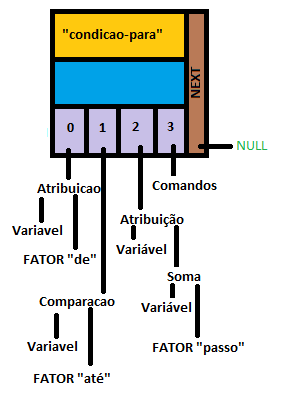
\includegraphics[width=0.4\textwidth]{imgs/Para.png}
\caption{\label{fig:para}Estrutura montada a partir do comando para.}
\end{figure}

\subsection{Se-ent\~ao e Se-ent\~ao-sen\~ao}

Um filho marca a compara\c{c}\~ao a ser realizada enquanto o segundo indica o que ser\'a realizado em caso de a condi\c{c}\~ao ser verdadeira, no caso de haver sen\~ao um terceiro filho guarda o que deve ser feito caso a condi\c{c}\~ao seja falsa. Ambos podem ser visto na figura \ref{fig:se}.

\begin{figure}
\centering
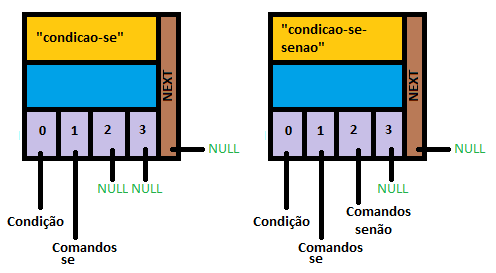
\includegraphics[width=0.5\textwidth]{imgs/se_e_se-senao.png}
\caption{\label{fig:se}Estruturas montadas a partir dos comandos se e se-sen\~ao.}
\end{figure}

\section{O interpretador}

\subsection{Funcionalidades}

O interpretador entregue prov\^e as seguintes funcionalidades: 

\begin{description}
\item[Compila\c{c}\~ao] S\~ao realizadas as etapas da an\'alise e s\'intese do programa apresentando os erros quando estes ocorrerem e, na ausencia de erros, montando toda a estrutura de execu\c{c}\~ao do programa;
\item[Execu\c{c}\~ao] \'E apresentada uma listagem com todos os programas compilados corretamente. Ao optar por um programa as respectivas estruturas deste s\~ao copiadas para o contexto de execu\c{c}\~ao e o mesmo \'e ent\~ao executado;
\item[Mostrar \'arvore de execu\c{c}\~ao] Exibe uma lista com todos os programas corretamente compilados e, para o selecionado, imprime sua \'arvore de execu\c{c}\~ao;
\item[Lista arquivos .gpt] Exibe uma listagem de todos os arquivos .gpt encontrados no diret\'orio atual.
\end{description}

\subsection{Interface}

\subsubsection{Apresenta\c{c}\~ao}

A tela de boas vindas, que dura 3 segundos, \'e apresentada na figura \ref{fig:apres}.

\begin{figure}
\centering
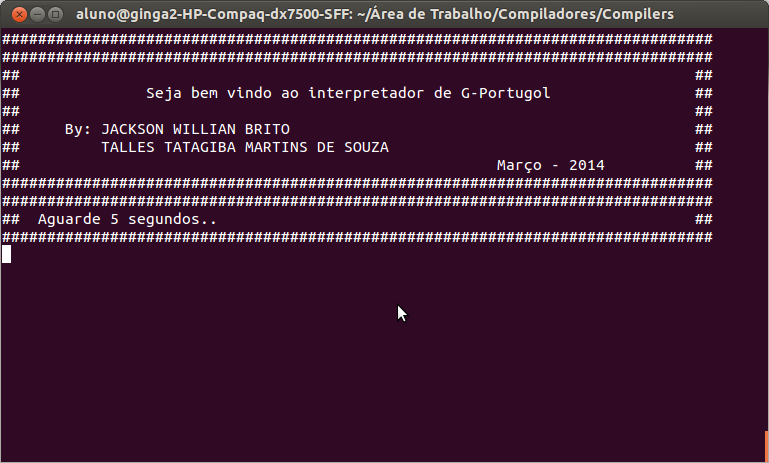
\includegraphics[width=0.6\textwidth]{imgs/Apresentacao.png}
\caption{\label{fig:apres}Tela de boas vindas do interpretador.}
\end{figure}

\subsubsection{Menu inicial}

A figura \ref{fig:menuinicial} apresenta a tela inicial do interpretador de onde pode-se selecionar a funcionalidade \`a qual deseja aceder.

\begin{figure}
\centering
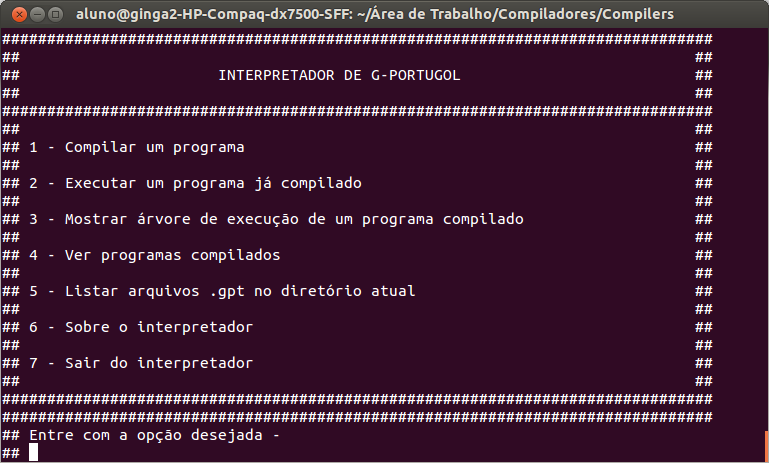
\includegraphics[width=0.6\textwidth]{imgs/menu_inicial.png}
\caption{\label{fig:menuinicial}Menu principal do interpretador.}
\end{figure}

\subsubsection{Compila\c{c}\~ao}

A figura \ref{fig:compilacao} mostra uma compila\c{c}\~ao que ocorreu com sucesso. Em caso de haver erros de compila\c{c}\~ao os mesmos seriam exibidos no lugar da mensagem de sucesso nessa tela.

\begin{figure}
\centering
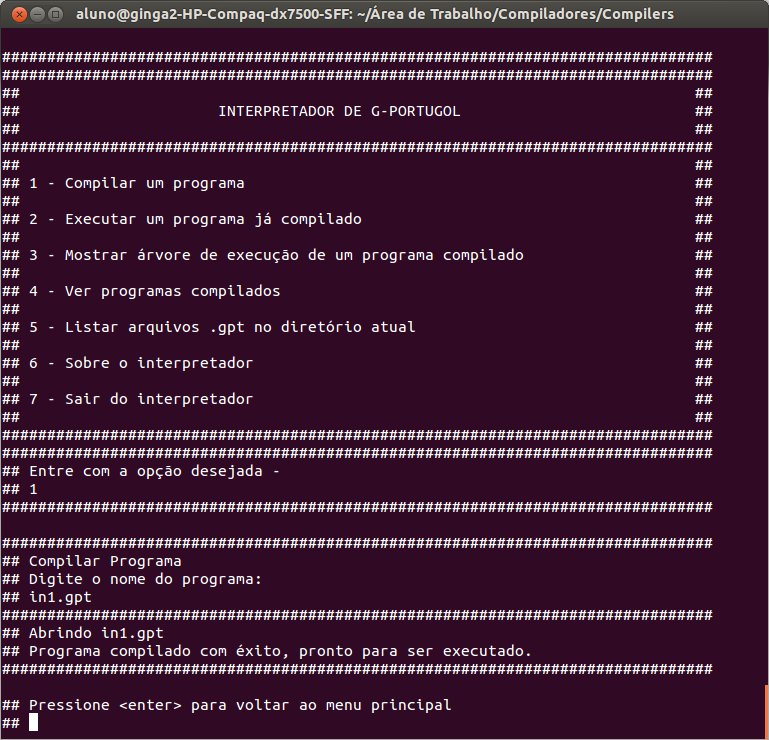
\includegraphics[width=0.6\textwidth]{imgs/Compilado.png}
\caption{\label{fig:compilacao}Exemplo de intera\c{c}\~ao na compila\c{c}\~ao de um programa.}
\end{figure}

\subsubsection{Execu\c{c}\~ao}

Um exemplo de execu\c{c}\~ao de um programa \'e mostrada na imagem \ref{fig:exec}.

\begin{figure}
\centering
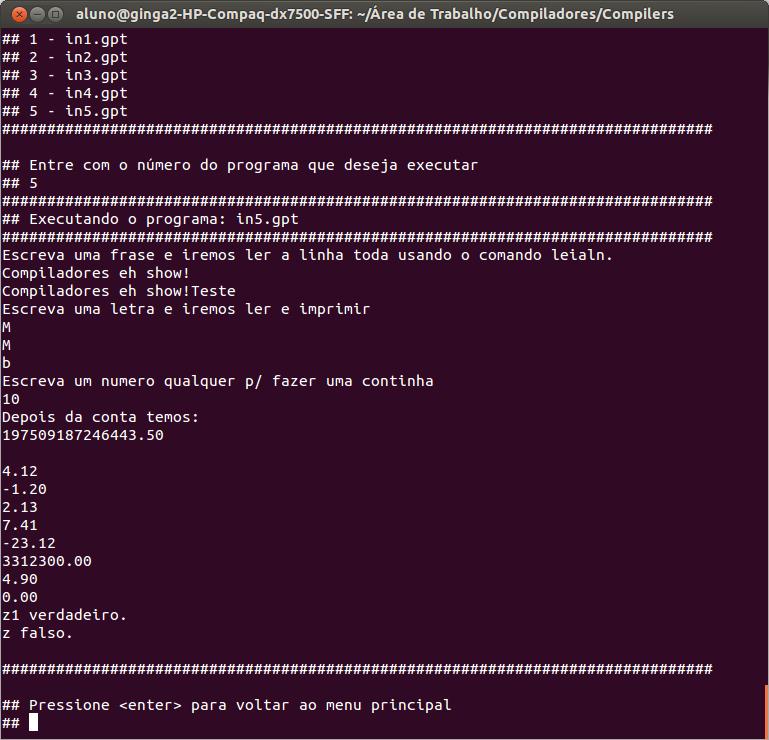
\includegraphics[width=0.6\textwidth]{imgs/Execucao_de_um_programa.png}
\caption{\label{fig:exec}Exemplo de intera\c{c}\~ao na execu\c{c}\~ao de um programa.}
\end{figure}

\subsubsection{Listar programas}

  Esta op\c{c}\~ao lista todos os programas compilado corretamente conforme visto na figura \ref{fig:listcomp}.

\begin{figure}
\centering
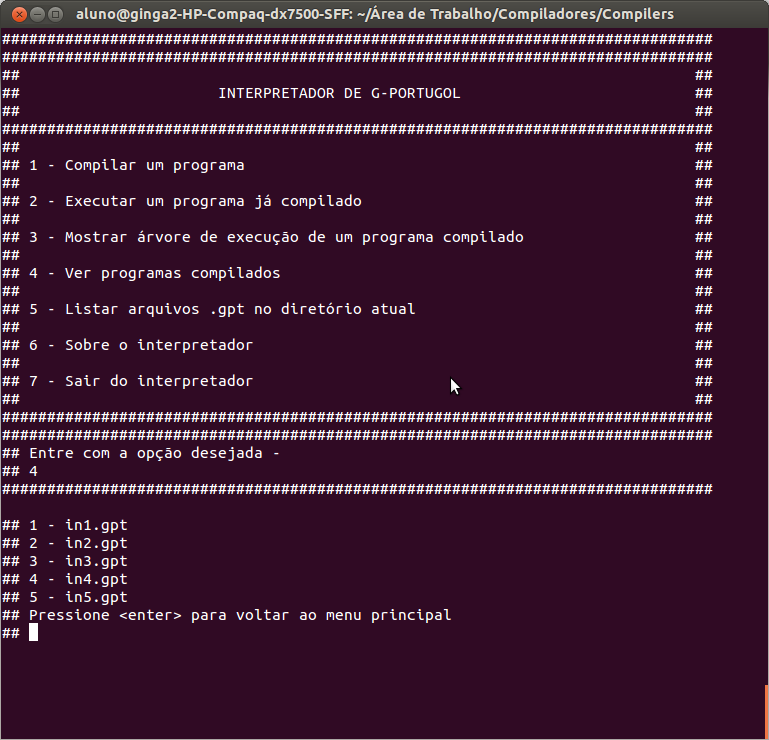
\includegraphics[width=0.6\textwidth]{imgs/Programas_compilados.png}
\caption{\label{fig:listcomp}Uma lista dos programas compilados com sucesso.}
\end{figure}

\subsubsection{Listar arquivos .gpt}

Esta op\c{c}\~ao lista todos os arquivos .gpt existentes no diret\'orio de execu\c{c}\~ao do interpretado. Um exemplo pode ser conferido na tela da figura \ref{fig:listarqv}.

\begin{figure}
\centering
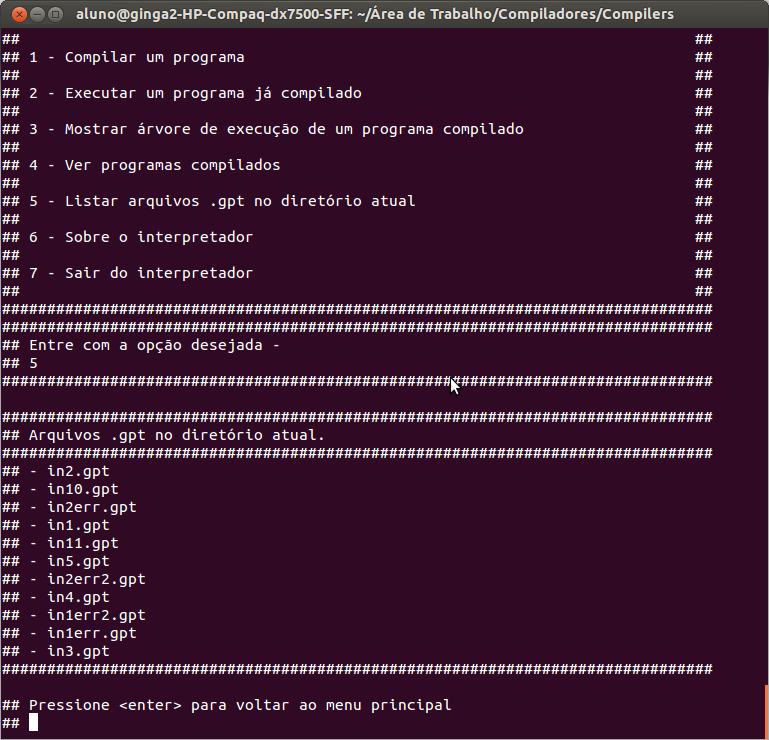
\includegraphics[width=0.6\textwidth]{imgs/Listar_programas.png}
\caption{\label{fig:listarqv}Uma lista dos programas candidatos a serem compilados no diret\'orio atual.}
\end{figure}

\subsubsection{Sobre}

Algumas informa\c{c}\~oes a respeito do interpretador podem ser conferidas na figura \ref{fig:sobre}.

\begin{figure}
\centering
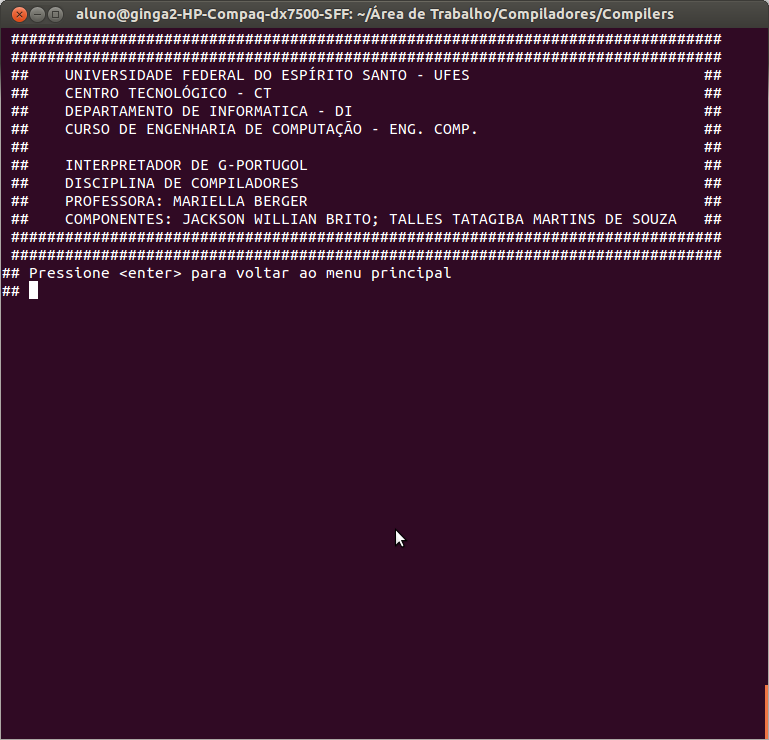
\includegraphics[width=0.6\textwidth]{imgs/Sobre.png}
\caption{\label{fig:sobre}Informa\c{c}\~oes a respeito do interpretador.}
\end{figure}

\subsubsection{Sauda\c{c}\~ao}

Ao fim do uso do nosso interpretador, emitimos uma sauda\c{c}\~ao a seu usu\'ario. Sauda\c{c}\~ao esta que pode ser vista na figura \ref{fig:sauda}

\begin{figure}
\centering
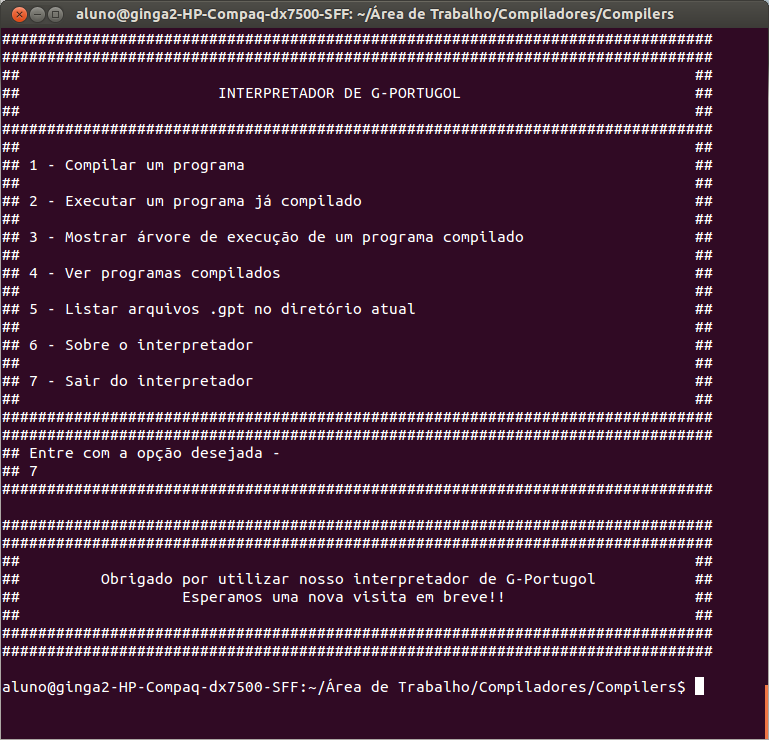
\includegraphics[width=0.6\textwidth]{imgs/Saudacao.png}
\caption{\label{fig:sauda}Cumprimentos ao usu\'ario.}
\end{figure}

\section{Casos de teste}

Conforme solicitado na especifica\c{c}\~ao do trabalho enviamos no diret\'orio exemplos 15
exemplos de programas escrito na linguagem portugol aceita pelo nosso compilador. 
Destes, 5 escritos de forma correta, 5 apresentando erros sint\'aticos e 5 com erros 
sem\^anticos.

\subsection{Testes corretos}

\subsubsection{in1.gpt}

Neste arquivo testamos o uso de atribui\c{c}\~oes e fun\c{c}\~oes recursivas.

\subsubsection{in2.gpt}

Neste arquivo testamos rigidamente o uso de condicionais e o aninhamento dos mesmos, para todos os casos, inclusive o \i{for}. Para verificar veracidade do algoritmo, v\'arias impress\~oes s\~ao realizadas durante o c\'odigo. 

\subsubsection{in3.gpt}

A estrutura do \i{switch-case} \'e testada com alguns caso e o condi\c{c}ao fa\c{c}a-enquanto tamb\'em. O uso das fun\c{c}~oes matem\'ativas primitivas da linguagem tamb\'em \'e explorado.

\subsubsection{in4.gpt}

Matrizes s\~ao intensamente testadas neste exemplo junto com um teste legal para impress\'~ao de primos que utiliza aninhamento de condicionais e repeti\c{c}\~oes. 

\subsubsection{in5.gpt}

As mastrizes s\~ao novamente testadas neste arquivo com o uso de fun\c{c}\~oes de IO primitivas da linguagem.


\subsection{Testes com erro: sem\^antica}

Os testes com erros s\~ao essencialmente os testes corretos com algum erro 
introduzido propositalmente
e abaixo descritos.

\subsubsection{in1err1.gpt}
Erro: Valores incompativeis na linha 43.
Valor do tipo real n\~ao pode ser utilizado junto com valores do tipo inteiro.

\subsubsection{in2err1.gpt}

Erro: Variavel variavel na linha 15 nao foi declarada.
Vari\'avel n\~ao foi declarada, portanto ocorre erro.

\subsubsection{in3err1.gpt}

Erro: Funcao maximo inteiro com aridade errada na linha 39.
A aridade da fun\c{c}\~ao primitiva m\'aximo da linguagem est\'a incorreta.


\subsubsection{in4err1.gpt}

Erro: Erro na linha 35, mat\_inteiro possui 5 linhas apenas.
O c\'odigo est\'a tentando acessa uma posi\c{c}\~ao da matriz que n\~ao existe.


\subsubsection{in5err1.gpt}

Erro: Atribuição de tipos invalidos na linha 42.
A atribui\c{c}~ao n\~ao \'e v\'alida porque o tipo da matriz \'e diferente.

\subsection{Testes com erro: sint\'atico}

Os testes com erros s\~ao essencialmente os testes corretos com algum erro 
introduzido propositalmente e abaixo descritos.

\subsubsection{in1err2.gpt}

Erro na Linha: 44
Est\'a faltando uma aspas dentro da fun\c{c}\~ao primitiva imprimir.

\subsubsection{in2err2.gpt}

Erro na Linha: 24
Est\'a faltando o final do condicional, fim-se.

\subsubsection{in3err2.gpt}

Erro na Linha: 54
Est\'a faltando algum FATOR dentro do caso.

\subsubsection{in4err2.gpt}

Erro na Linha: 35
Est\'a faltando um colchete na matriz.

\subsubsection{in5err2.gpt}

Erro na Linha: 34
Est\'a faltando um par\^enteses na express\~ao.

\section{Conclus\~ao}

Este trabalho exigiu muito tempo dos integrantes, mas ao final se provou bem satisfat\'orio. Nele solidificou-se o conhecimento nas tr\^es etapas de an\'alise de uma linguagem de programa\c{c}\~ao, l\'exica, sint\'atica e sem\^antica e da cria\c{c}\~ao de um interpretador atrav\'es do uso de uma linguagem intermedi\'aria baseada em estruturas de dados de \'arvores e posterior execu\c{c}\~ao. 


\end{document}